\documentclass{article}
\usepackage[spanish]{babel}
\usepackage{graphicx}
\usepackage{subfigure}
\graphicspath{{/home/vian/0_uam/1_TFG/latex/resultados/img/}}

\title{integracion, pruebas y resultados}
\author{Yo}

\begin{document}
\maketitle{}
\tableofcontents{}

\newpage

% TODO: Hacer introducción a los resultados (explicar lo que se va a mostrar y tal vez cómo)
% TODO: Mostrar resultados en tablas comparativas, agrupando por grafo y cambiando los modificadores (al menos una vez para enseñar qué cambio hay) y tal vez de forma anecdótica la modificación de P (lagrange_multiplier en DWave). Después de mostrar las diferencias entre distintas versiones de Qiskit, mostrar la que mejor quede con el caso de DWave. También mostrar las diferentes métricas (max statistics, global y gamma function)
A continuación se mostrarán los resultados de ejecución utilizando ambos paradigmas, esto es, QAOA y Quantum Annealing, además de explorar el rendimiento de las ejecuciones en Qiskit variando los métodos para construir la función de coste.

\section{Primer grafo}
\label{sec:primer-grafo}

\begin{figure}[htbp]
  \centering
  \includegraphics[scale=0.75]{primer_grafo/primer_grafo}
  \caption{Grafo del artículo original} \label{fig:primer_grafo/primer_grafo}
\end{figure}

% Tabla de ejemplo:
% \begin{table}[htbp]
%   \centering
%   \begin{tabular}{|c|r|r|l|}  % r == right, l == left, c == center
%     \hline
%     \textbf{Qubits} & \textbf{Camino} & \textbf{Frecuencia} & Izda \\
%     \hline
%     10101 & hola & 917 & a \\
%     10110 & hola & 82 & a \\
%     01001 & hola & 1 & a \\
%     \hline
%   \end{tabular}
%   \label{tab:ejemplo}
%   \caption{captionada}
% \end{table}
% Tabla referenciada: \ref{tab:ejemplo}

\subsection{Resultados de Qiskit}
\label{sec:resultados-de-qiskit}
\subsubsection{Primer grafo}

Sobre los dos tipos de medición de estadísticas: \\
% TODO: Hablar aquí sobre la diferencia entre los modificadores y la restricción extra
En las siguientes muestras se ha buscado replicar los resultados del artículo. Esto ha sido probado dado que, empleando los parámetros \(\beta = 0.28517317\) y \(\gamma = -5.05969577 \) dados como óptimos, se obtiene un gráfico muy similar al dado: \\

% TODOOO: Mostrar ambos gráficos, el del paper original y el mío
\begin{figure}[htbp]
  \centering
  \subfigure[Resultado del artículo]{
    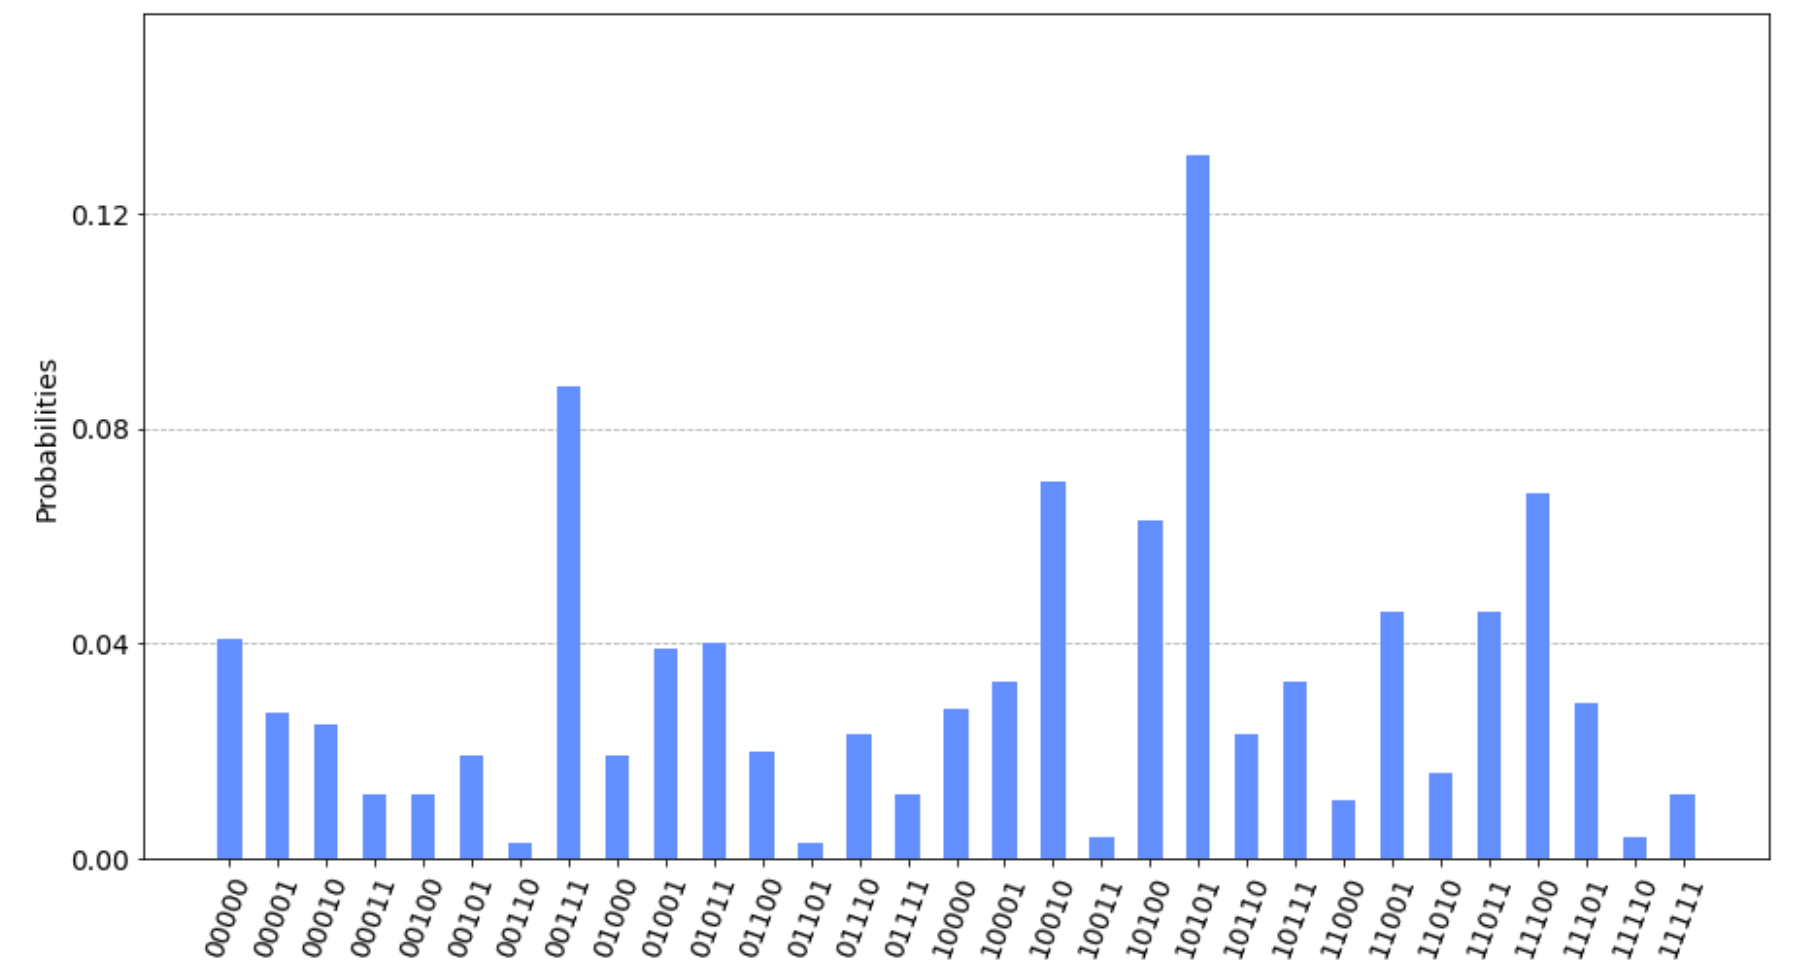
\includegraphics[width=0.475\textwidth]{primer_grafo/sin_restriccion_extra/primer_paper_orig_resultado}
  }
  \subfigure[Resultado obtenido]{
    \includegraphics[width=0.475\textwidth]{primer_grafo/sin_restriccion_extra/primer_paper_aer_resultado}
  }
  \caption{} \label{fig:primer_grafo/sin_restriccion_extra/primer_paper_aer_resultado}
\end{figure}

% 1000 Ejecuciones, no varía demasiado el resultado
% [('10101', 0.3934208984375), ('10001', 0.202630859375), ('00101', 0.046755859375), ('10110', 0.0414072265625), ('11001', 0.0325322265625), ('00001', 0.0323759765625), ('11101', 0.0298798828125), ('10100', 0.0293173828125), ('10111', 0.028814453125), ('10010', 0.028650390625), ('10000', 0.0264873046875), ('10011', 0.022994140625), ('00111', 0.0122685546875), ('00011', 0.00875390625), ('01001', 0.0068291015625), ('00000', 0.0066201171875), ('11011', 0.0057099609375), ('00010', 0.005537109375), ('00100', 0.0050537109375), ('11100', 0.00461328125), ('11000', 0.00444921875), ('01101', 0.00444921875), ('00110', 0.004314453125), ('11111', 0.0042646484375), ('11010', 0.0037236328125), ('01011', 0.0023720703125), ('01111', 0.0014287109375), ('01000', 0.0012861328125), ('11110', 0.001181640625), ('01100', 0.000876953125), ('01010', 0.0006611328125), ('01110', 0.00033984375)]

% {'10110': 75, '10101': 925}

También se han realizado pruebas sobre la diferencia entre varias métricas distintas con las que medir la eficacia de los resultados.
\begin{itemize}
\item Estadística máxima:
  Con este método se busca obviar el ruido presente en cada ejecución. Para ello se realizan \textit{n} iteraciones distintas sobre el algoritmo, y para cada una de ellas:
  \begin{enumerate}
  \item Se ejecuta el optimizador clásico para hallar los parámetros óptimos (esto supone la ejecución del circuito cuántico el número de veces necesario para que el optimizador encuentre un mínimo local).
  \item Se ejecuta el circuito una vez más con los parámetros óptimos.
  \item \label{it:estadistica_max} Se obtiene el camino dado por el algoritmo para recorrer el grafo y se añade dicho camino a un diccionario para su posterior revisión. En el caso de la figura \ref{fig:primer_grafo/sin_restriccion_extra/primer_paper_aer_resultado}
    el resultado sería \textit{10101}, es decir, el camino con mayor valor.
  \end{enumerate}
\item Estadística global:
  A diferencia de la estrategia previamente explicada, al realizar el paso \ref{it:estadistica_max} se toman todos los caminos resultantes de la ejecución del circuito con los parámetros \(\beta_{opt}\) y \(\gamma_{opt}\).
  De esta forma, una ejecución como la dada en la figura \ref{fig:primer_grafo/sin_restriccion_extra/primer_paper_aer_resultado}
  se ve condicionada por todos los resultados, no únicamente por el camino con valor máximo.
\item Función gamma:  % TODOO: Explicar gamma function
\end{itemize}

\end{document}
%%% Local Variables:
%%% mode: latex
%%% TeX-master: t
%%% End:
